% PLEASE USE THIS FILE AS A TEMPLATE
% Check file iosart2c.tex for more examples
%
% Journal:
%   Journal of Ambient Intelligence and Smart Environments (jaise)
%   Web Intelligence and Agent Systems: An International Journal (wias)
%   Semantic Web: Interoperability, Usability, Applicability (SW)
% IOS Press
% Latex 2e

% options: jaise|wias|sw
% add. options: [seceqn,secfloat,secthm,crcready,onecolumn]


\documentclass{iosart2c}

%\documentclass[sw]{iosart2c}
%\documentclass[wias]{iosart2c}
%\documentclass[jaise]{iosart2c}

\usepackage[T1]{fontenc}
\usepackage{times}%
\usepackage{natbib}% for bibliography sorting/compressing
%\usepackage{amsmath}
%\usepackage{endnotes}
\usepackage{graphicx}

%%%%%%%%%%% Put your definitions here
\usepackage[utf8]{inputenc}
\usepackage[hyphens]{url}
\usepackage{verbatim} 
\usepackage[pdftex,urlcolor=black,colorlinks=true,linkcolor=black,citecolor=black,draft]{hyperref}
\def\sectionautorefname{Section}
\def\subsectionautorefname{Subsection}
\usepackage{listings}
\usepackage{textcomp}
\lstset{
        basicstyle=\ttfamily\scriptsize,
        upquote=true,
        showspaces=false,
        showstringspaces=false,
        showtabs=false,
        tabsize=2,
        frame=none,
        breaklines,
        numbers=none,
        framexleftmargin=2mm,
        xleftmargin=2mm,
}

% bullet numbers
\usepackage{tkz-graph}
\usetikzlibrary{matrix,arrows,decorations.pathmorphing,shapes}
\newcommand{\dobulletnumber}[1]{\node[circle,text=white,fill=gray,anchor=west,inner sep=1pt] {\sffamily #1}}
\newcommand{\bulletnumber}[1]{\tikz[baseline=-2.5,overlay]\dobulletnumber{#1};}
\newcommand{\bulletref}[1]{\tikz[baseline=-2.5]\dobulletnumber{\fontsize{8}{8}\selectfont#1};}
% todo macro
\usepackage{color}
\newcommand{\todo}[1]{\noindent\textcolor{red}{{\bf \{TODO}: #1{\bf \}}}}

%% Define a new 'smallurl' style for the package that will use a smaller font.
\makeatletter
\def\url@smallurlstyle{%
  \@ifundefined{selectfont}{\def\UrlFont{\sf}}{\def\UrlFont{\scriptsize\ttfamily}}}
\makeatother
%% Now actually use the newly defined style.
\urlstyle{smallurl}
\newcommand{\nofootnote}[1]{~#1}

%%%%%%%%%%% End of definitions

\pubyear{0000}
\volume{0}
\firstpage{1}
\lastpage{1}

\begin{document}

\begin{frontmatter}

\pretitle{What'chu talkin' about, Willis?}
\title{A comparison of topics people read about on Facebook and Twitter, and where they are}
%\subtitle{}

%\footnote{\url{http://en.wikipedia.org/wiki/Diff'rent\_Strokes\#Later\_appearances\_of\_the\_characters}}

\runningtitle{A comparison of topics people read about on Facebook and Twitter, and where they are}

%\review{}{}{}

% Two or more authors:
\author[A]{\fnms{Thomas} \snm{Steiner}\thanks{T. Steiner is partially supported by the European Commission under Grant No. 248296 FP7 I-SEARCH project}},
\author[B]{\fnms{Ruben} \snm{Verborgh}},
\author[A]{\fnms{Arnaud} \snm{Brousseau}\thanks{A. Brousseau was an intern at Google Germany GmbH at the time of writing.}},
\author[C]{\fnms{Raphaël} \snm{Troncy}},
\author[B]{\fnms{Rik} \snm{Van de Walle}},
\author[D]{\fnms{Joaquim} \snm{Gabarró Vallés}}

\runningauthor{T. Steiner, A. Brousseau, R. Troncy, R. Verborgh, et al.}

\address[A]{Google Germany GmbH, ABC-Str. 19, 20354 Hamburg, Germany,\\
E-mail: tomac@google.com, arnaud.brousseau@gmail.com}
\address[B]{Ghent University -- IBBT, ELIS, Multimedia Lab, Gaston Crommenlaan 8/201, 9050 Ghent, Belgium,\\
E-mail: ruben.verborgh@ugent.be, rik.vandewalle@ugent.be}
\address[C]{EURECOM, Sophia Antipolis, France\\
E-mail: raphael.troncy@eurecom.fr}
\address[D]{Universitat Polit\`{e}cnica de Catalunya, Department LSI, 08034 Barcelona, Spain,\\
E-mail: gabarro@lsi.upc.edu}

\begin{abstract}
\todo{Write abstract}
\end{abstract}

\begin{keyword}
\todo{List keywords}
\end{keyword}

\end{frontmatter}

%%%%%%%%%%% The article body starts:

\section{Introduction} \label{sec:introduction}
\subsection{On Social Media Mining}
In recent years, social media mining has become an essential tool for marketers, traders, and researchers.
The information people share publicly via so-called \emph{microposts} on social networks harbor tremendous amounts of valuable social data.
Forbes has called the social graph \emph{crude oil} in a recent blog post~\cite{ForbesPost}.
Social networks today are very much ``walled gardens'', excellently illustrated by a cartoon by David Simonds~(\autoref{fig:DavidSimonds}).
This network isolatedness reflects on how social media mining is done nowadays.
Common literature typically either focuses on just one network~(e.g.,~\cite{russell201121}), or treats the different networks separately~(e.g.,~\cite{russell2011mining}).
Social media mining happens based on either keyword-based search APIs, or so-called ``fire hose'' near-realtime streaming APIs, both provided by the social networks themselves.
The main difference is that in the prior case terms like the name of a brand or company are \emph{proactively} searched for, whereas in the latter case the social media mining system \emph{reactively} acts upon the occurrence of such terms.

\subsection{Selection of Social Networks and APIs}
In this paper, we consider the popular social networks Facebook\footnote{\url{http://facebook.com/}} and Twitter\footnote{\url{http://twitter.com/}}, currently the two globally most important social networks~\cite{comScoreTwitter, comScoreFacebook}.
Traditionally, Twitter is very open with their API, as since the beginning of the platform, API-based Twitter clients  play a strategic role for the company.
Twitter provides developers with the Twitter Streaming API~\cite{TwitterStreamingAPI}, which allows for high-throughput near-realtime access to various subsets of public and protected Twitter data.
Facebook has no such public ``fire hose'' API, however, via its Graph API~\cite{FacebookRealtimeAPI} supports near-realtime updates to enable applications to subscribe to a limited set of changes in data from Facebook.
Whenever such a change occurs, Facebook notifies subscribers with a list of changes.
The obvious issue here is that, in order to get a Twitter Streaming API-like experience, one had to subscribe to a high number of users, which is impossible.
This imbalance of API openness has an impact on academic publications around mining social networks.
While at the \textit{World Wide Web Conference 2011} alone three Twitter papers based on the Twitter API were published~\cite{Meeder:2011:WKY:1963405.1963479, Romero:2011:DMI:1963405.1963503, Wu:2011:SWT:1963405.1963504}, publications on Facebook typically focus on privacy issues~(e.g.,~\cite{liu:settings}), or Facebook's sociological impact~(e.g.,~\cite{JCC4:JCC4367}), without making use of the Facebook API.

\subsection{Positioning of our Work}
What, to the best of our knowledge, all publications so far have in common is their focus on the author side: it is very well researched what people \emph{produce} on social networks (especially Twitter), whom they follow or unfollow and why, what they tag, whom they put in what list, group, or circle. However, few to no focus has been given on what people \emph{consume} -- or at least no such study is publicly available.
This is especially true \emph{across} social networks.
As far as we can tell, no study has compared \emph{reader} behavior on \emph{different} social networks before.
In this work, we thus compare topics people read about on Facebook and on Twitter, and classify those topics in order to provide an overall comparison. 
We therefore have implemented two similar browser extensions: Twitter Swarm NLP\footnote{\url{http://bit.ly/twitterswarmnlp}} and Facebook Swarm NLP\footnote{\url{http://bit.ly/facebookswarmnlp}}. 
On the one hand, these extensions enrich the user experience on those two social networks and on the other hand, they determine the topics that people see and read about on their timelines by means of named entity disambiguation.
We combine this knowledge with additional anonymous data that we obtain about social network users.
In consequence, on the other hand, the extensions gather anonymous visitor information via a common Web analytics tool.

\subsection{Focus on Desktop Versions}
By focusing exclusively on content people see when directly navigating to the desktop versions of either \url{http://twitter.com} or \url{http://facebook.com} (and in consequence on purpose neglecting all activity via applications), we assume people indeed read that content, especially as both social network sites require users to actively click a link ``$\mathit{n}$ new stories'' (Facebook) or ``$\mathit{n}$ new tweets'' (Twitter) rather than auto-updating the timeline.
Other approaches to determine whether a micropost has been read are limited to microposts with contained Web links and checking whether clicks on those links have occurred, however, automatic crawling and indexing of links adds hard to detect noise.
We argue that our approach has a higher precision, however, less recall.

\subsection{Paper Objective and Structure}
We outline or paper objectives and non-objectives implicitly, where  each objective has a corresponding non-objective in the two lists below.

\noindent In this paper, we \textbf{will}:
\begin{itemize}%[topsep=-.5em, partopsep=0pt, itemsep=0pt]
	\item perform analyses based on disambiguated named entities;
	\item perform analyses based on IP-based reader location detection;
	\item work with a manageable amount of microposts read by a random population of social network users;
	\item focus on the micropost reader side.
\end{itemize}
On the contrary, we \textbf{will not}:
\begin{itemize}%[topsep=-.5em, partopsep=0pt, itemsep=0pt]
	\item perform analyses based on hashtags, key term frequencies, or trends;
	\item perform analyses based on geotagged microposts;
	\item work with huge amounts of microposts from ``fire hose'' APIs;
	\item focus on the micropost author side,
\end{itemize}
which is why we strive for a paradigm shift that promises new insights for tasks like brand analysis, opinion research, but also sociological questions.

\todo{Describe paper structure.}

\begin{figure}
\centering
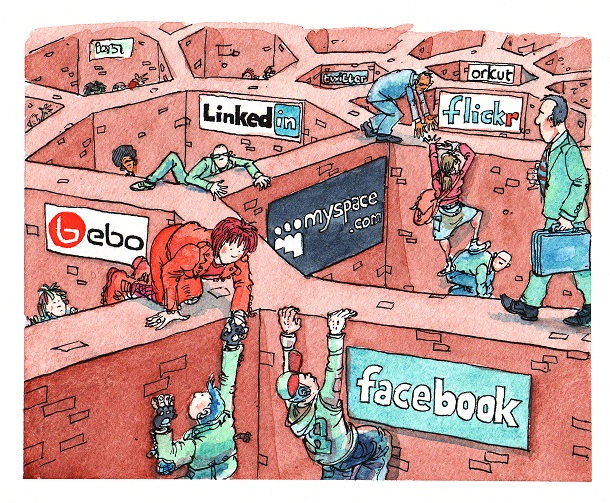
\includegraphics[width=1.0\linewidth]{./resources/davidsimonds.png}
\caption{Social networks as walled gardens.~\cite{DavidSimonds}}
\label{fig:DavidSimonds}
\end{figure}

\section{Implementation} \label{sec:implementation}
\subsection{Structuring Unstructured Data}    \label{sec:services}
Sir Tim Berners-Lee has introduced Linked Data in a W3C Design Issue~\cite{TimBL:LinkedData}, where he defines the four rules for Linked~Data:
\begin{enumerate}
\item Use URIs as names for things.
\item Use HTTP URIs so that people can look up those names.
\item When someone looks up a URI, provide useful information, using the standards (RDF*, SPARQL).
\item Include links to other URIs, so that they can discover more things.
\end{enumerate}
In order to represent extracted named entities from microposts in an unambiguous way, we apply the first and the second Linked Data principle by representing disambiguated named entities with HTTP URIs.
We outsource this task to third party named entity disambiguation Web services, namely OpenCalais~\cite{OpenCalais}, Zemanta~\cite{Zemanta}, DBpedia Spotlight~\cite{Spotlight}, and AlchemyAPI~\cite{AlchemyApi}.
These APIs take a text fragment as input, perform named entity extraction and disambiguation on it, and then link the extracted entities back into the Linking Open Data (LOD) cloud~\cite{LODcloud}.
We use these APIs in parallel and, by combining their results, aim at the emergence effect in the sense of Aristotle: ``\emph{[\ldots] the totality is not, as it were, a mere heap, but the whole is something besides the parts [\ldots]}''\footnote{Aristotle, Metaphysics, Book H 1045a 8-10.}. 

\subsection{Combining Results from different APIs}                     \label{sec:consolidation-nlp}
We have implemented a wrapper API for the four named entity disambiguation APIs introduced in~\autoref{sec:services}.
While the original calls to each particular API are all HTTP \texttt{POST}-based, we have implemented the wrapper API \texttt{GET}-based, which is not an issue given limited micropost lengths.
It returns results in \texttt{application/json} format.
While the underlying APIs return entities with their types and/or subtypes, names, relevance, and URIs that link into the LOD cloud in different formats, the wrapper API abstracts away the different output formats and returns a common JSON object structure instead.
The output in JSON form for an exemplary micropost can be seen in~\autoref{lst:nlpjson}.

\begin{lstlisting}[caption={Named entity disambiguation wrapper API output in JSON form for the micropost \textit{``Tom has the LaTeX, BibTeX, LaTeX, LaTeX blues...''}.},label={lst:nlpjson}]
[
    {
        "name": "LaTeX",
        "relevance": 0.2500259280204773,
        "uris": [
            {
                "uri": "http://dbpedia.org/resource/LaTeX",
                "source": "spotlight"
            }
        ],
        "source": "spotlight"
    },
    {
        "name": "BibTeX",
        "relevance": 0.5101502607741356,
        "uris": [
            {
                "uri": "http://rdf.freebase.com/ns/en/bibtex",
                "source": "zemanta"
            },
            {
                "uri": "http://dbpedia.org/resource/BibTeX",
                "source": "zemanta"
            }
        ],
        "source": "zemanta,spotlight"
    },
    {
        "name": "blues",
        "relevance": 0.831137,
        "uris": [
            {
                "uri": "http://rdf.freebase.com/ns/en/blues",
                "source": "zemanta"
            },
            {
                "uri": "http://dbpedia.org/resource/Blues",
                 "source": "zemanta"
            }
        ],
        "source": "zemanta"
    }    
]
\end{lstlisting}

\subsection{Manipulating Web Pages with Browser Extensions}
Our approach is based on browser extensions.
Browser extensions are small software programs written in a combination of HTML, JavaScript, and CSS.
For this paper, we focus on extensions based on so-called content scripts.
Content scripts are JavaScript programs that run in the context of Web pages via dynamic code injection.
By using the standard Document Object Model (DOM), they can read or modify details of the Web pages a user visits.
The advantage of using browser extensions is that the concept is very powerful and generalizable at the same time.
Powerful in the sense that it allows for significantly changing one's user experience with social networking platforms like Twitter or Facebook and simply add new features.
Generalizable in the sense that the approach is expandable to more social networking platforms like MySpace~\cite{MySpace}, LinkedIn~\cite{LinkedIn}, Google+~\cite{GooglePlus}, etc. in the future.

\subsection{Gathering Visitor Data with Web Analytics Software}
In order to gather high-level information on Web page visitors apart from low-level log file statistics, so-called Web analytics software can used.
Such software is typically implemented by adding an invisible snippet of JavaScript code on the to-be-tracked pages of a website.
This code then collects visitor data through requests for a specific $\mathit{1} \times \mathit{1}$ transparent gif image, also called Web beacon, that is hosted on the Web analytics server.
During these requests the page and user data is reported in the query part of the Web beacon's URL.
In addition to that, the JavaScript snippet usually sets a first party cookie on visitors' computers in order to store anonymous information such as the timestamp of the current visit, whether the visitor is a new or returning visitor, and the referrer of the website that the visitor came from.
Part of the shared visitor information is the IP address, which allows for IP-based geolocation.

\begin{figure}
\centering
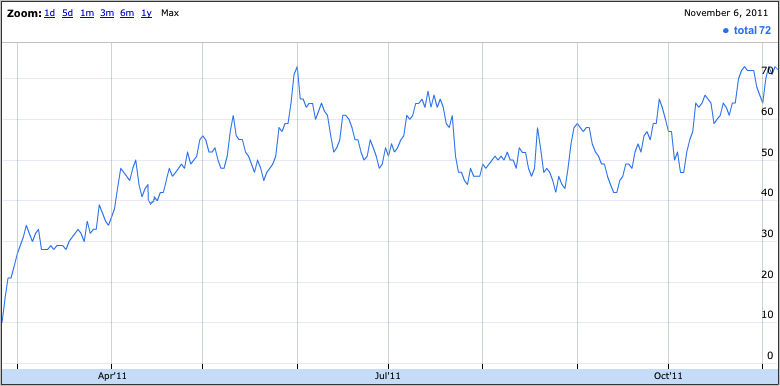
\includegraphics[width=1.0\linewidth]{./resources/twitterswarmnlpstats.png}
\caption{\textit{Seven day active users} development for the Twitter Swarm NLP browser extension.}
\label{fig:twitterswarmnlpstats}
\end{figure}

\begin{figure}
\centering
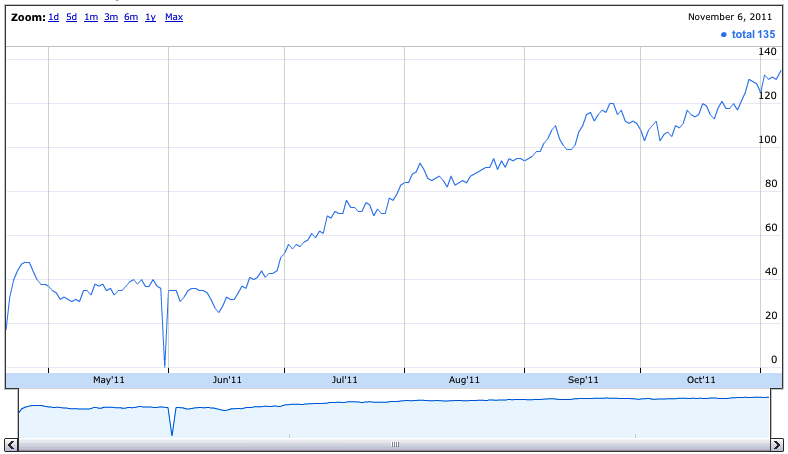
\includegraphics[width=1.0\linewidth]{./resources/facebookswarmnlpstats.png}
\caption{\textit{Seven day active users} development for the Facebook Swarm NLP browser extension.}
\label{fig:facebookswarmnlpstats}
\end{figure}

\section{User Demographics} \label{sec:userdemographics}
We have released the two browser extensions independently from each other on the Chrome Web Store.
The extension descriptions contain full disclosure on the collected data and on the usage of a Web analytics tool.
As the extensions inject a Web analytics tracking snippet, exact user localization is possible based on the users' current physical location, i.e., completely independent from the origin location users might have registered with Twitter or Facebook.
A graphical overview of user locations can be seen in~\autoref{fig:twitterlocation} and~\autoref{fig:facebooklocation}.
\autoref{tab:facebooklocations} and \autoref{tab:twitterlocations} show the distribution of the top-10 locations of users of the extensions.
The complete statistics can be found online\footnote{\url{https://github.com/tomayac/swj-microposts/tree/master/stats}}.

In the period from March~1 to November~8, for Facebook Swarm NLP, overall 858~unique Facebook users accessed the extension at least 10~times, in comparison to overall 86 unique Twitter Swarm NLP users.
If we put these figures in contrast with the \emph{seven day active users} statistics for the extensions~(\autoref{fig:facebookswarmnlpstats} and \autoref{fig:twitterswarmnlpstats}), where Facebook reached~135 and Twitter Swarm NLP 72~seven~day active users as of November~6, we can derive that Twitter users mostly installed the extension and stayed with it, whereas Facebook users installed the extension, used it for a while, and uninstalled it.

\begin{figure}
\centering
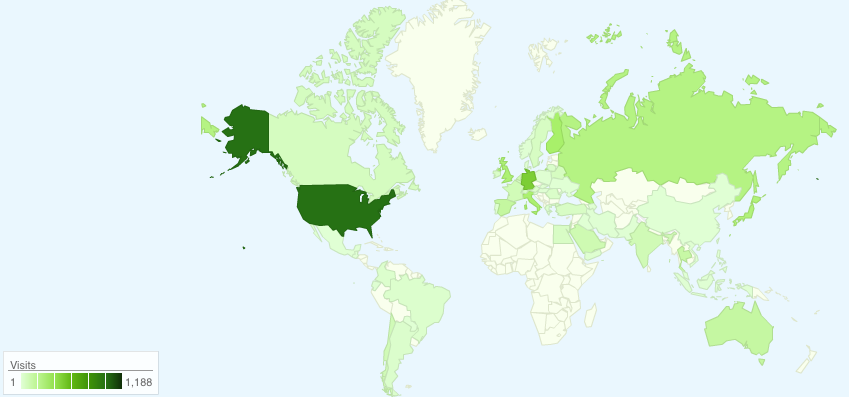
\includegraphics[width=1.0\linewidth]{./resources/twitterlocation.png}
\caption{Location of users of the Twitter Swarm NLP browser extension (May 1 -- Nov. 12).}
\label{fig:twitterlocation}
\end{figure}

\begin{figure}
\centering
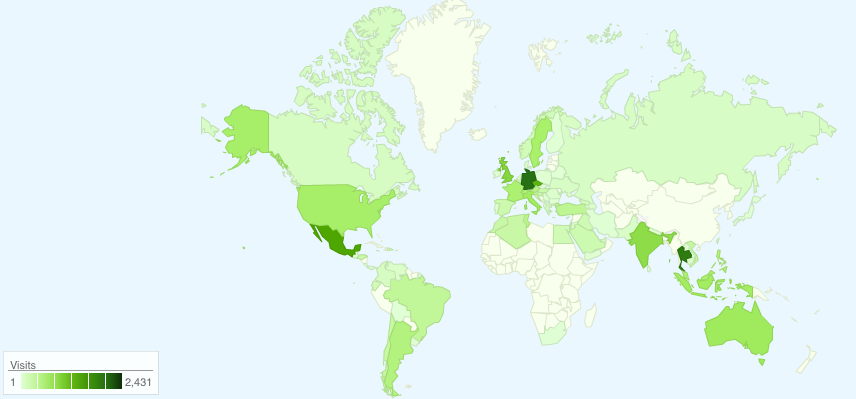
\includegraphics[width=1.0\linewidth]{./resources/facebooklocation.png}
\caption{Location of users of the Facebook Swarm NLP browser extension (May 1 -- Nov. 12).}
\label{fig:facebooklocation}
\end{figure}

\begin{figure}
\centering
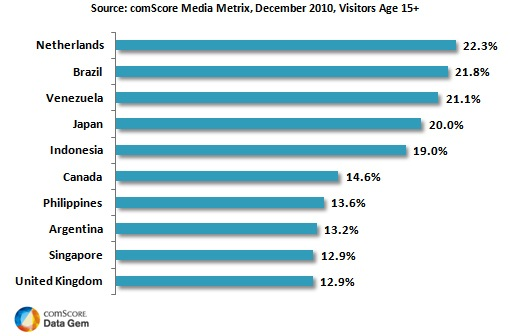
\includegraphics[width=1.0\linewidth]{./resources/twitterglobalmarkets.jpg}
\caption{Twitter Global Markets Reach. Source:~\cite{comScoreTwitter}.}
\label{fig:twitterglobalmarkets}
\end{figure}

\begin{figure}
\centering
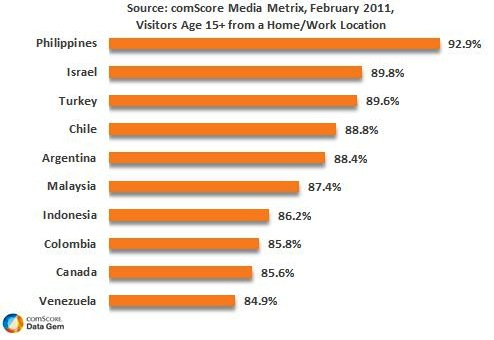
\includegraphics[width=1.0\linewidth]{./resources/facebookglobalmarkets.jpg}
\caption{Facebook Global Markets Reach. Source:~\cite{comScoreFacebook}.}
\label{fig:facebookglobalmarkets}
\end{figure}

\begin{figure*}
\centering
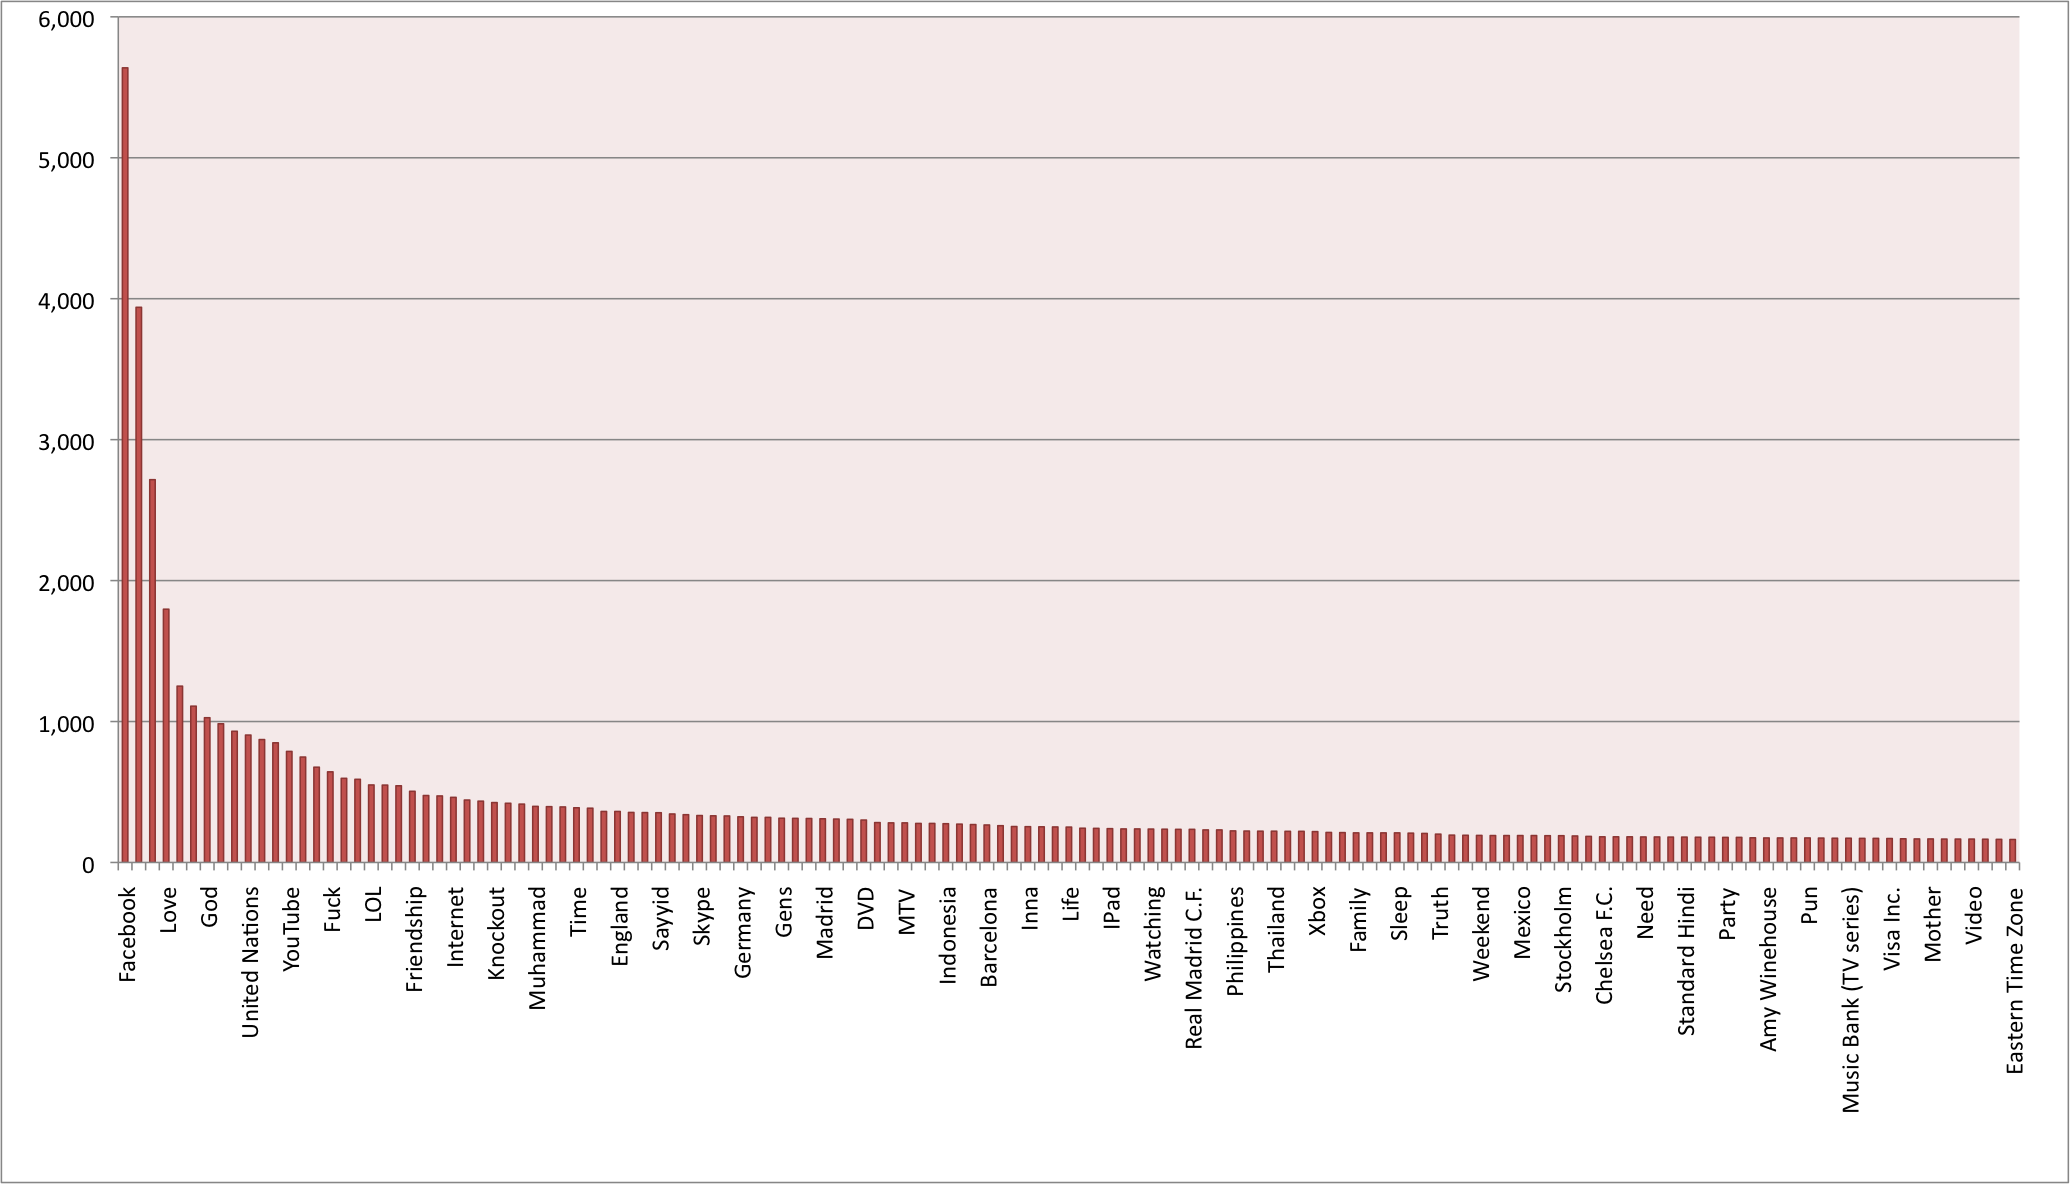
\includegraphics[width=1.0\linewidth]{./resources/facebooktopentities.png}
\caption{Facebook top entities as reported by Facebook Swarm NLP users.}
\label{fig:facebooktopentities}
\end{figure*}

\begin{figure*}
\centering
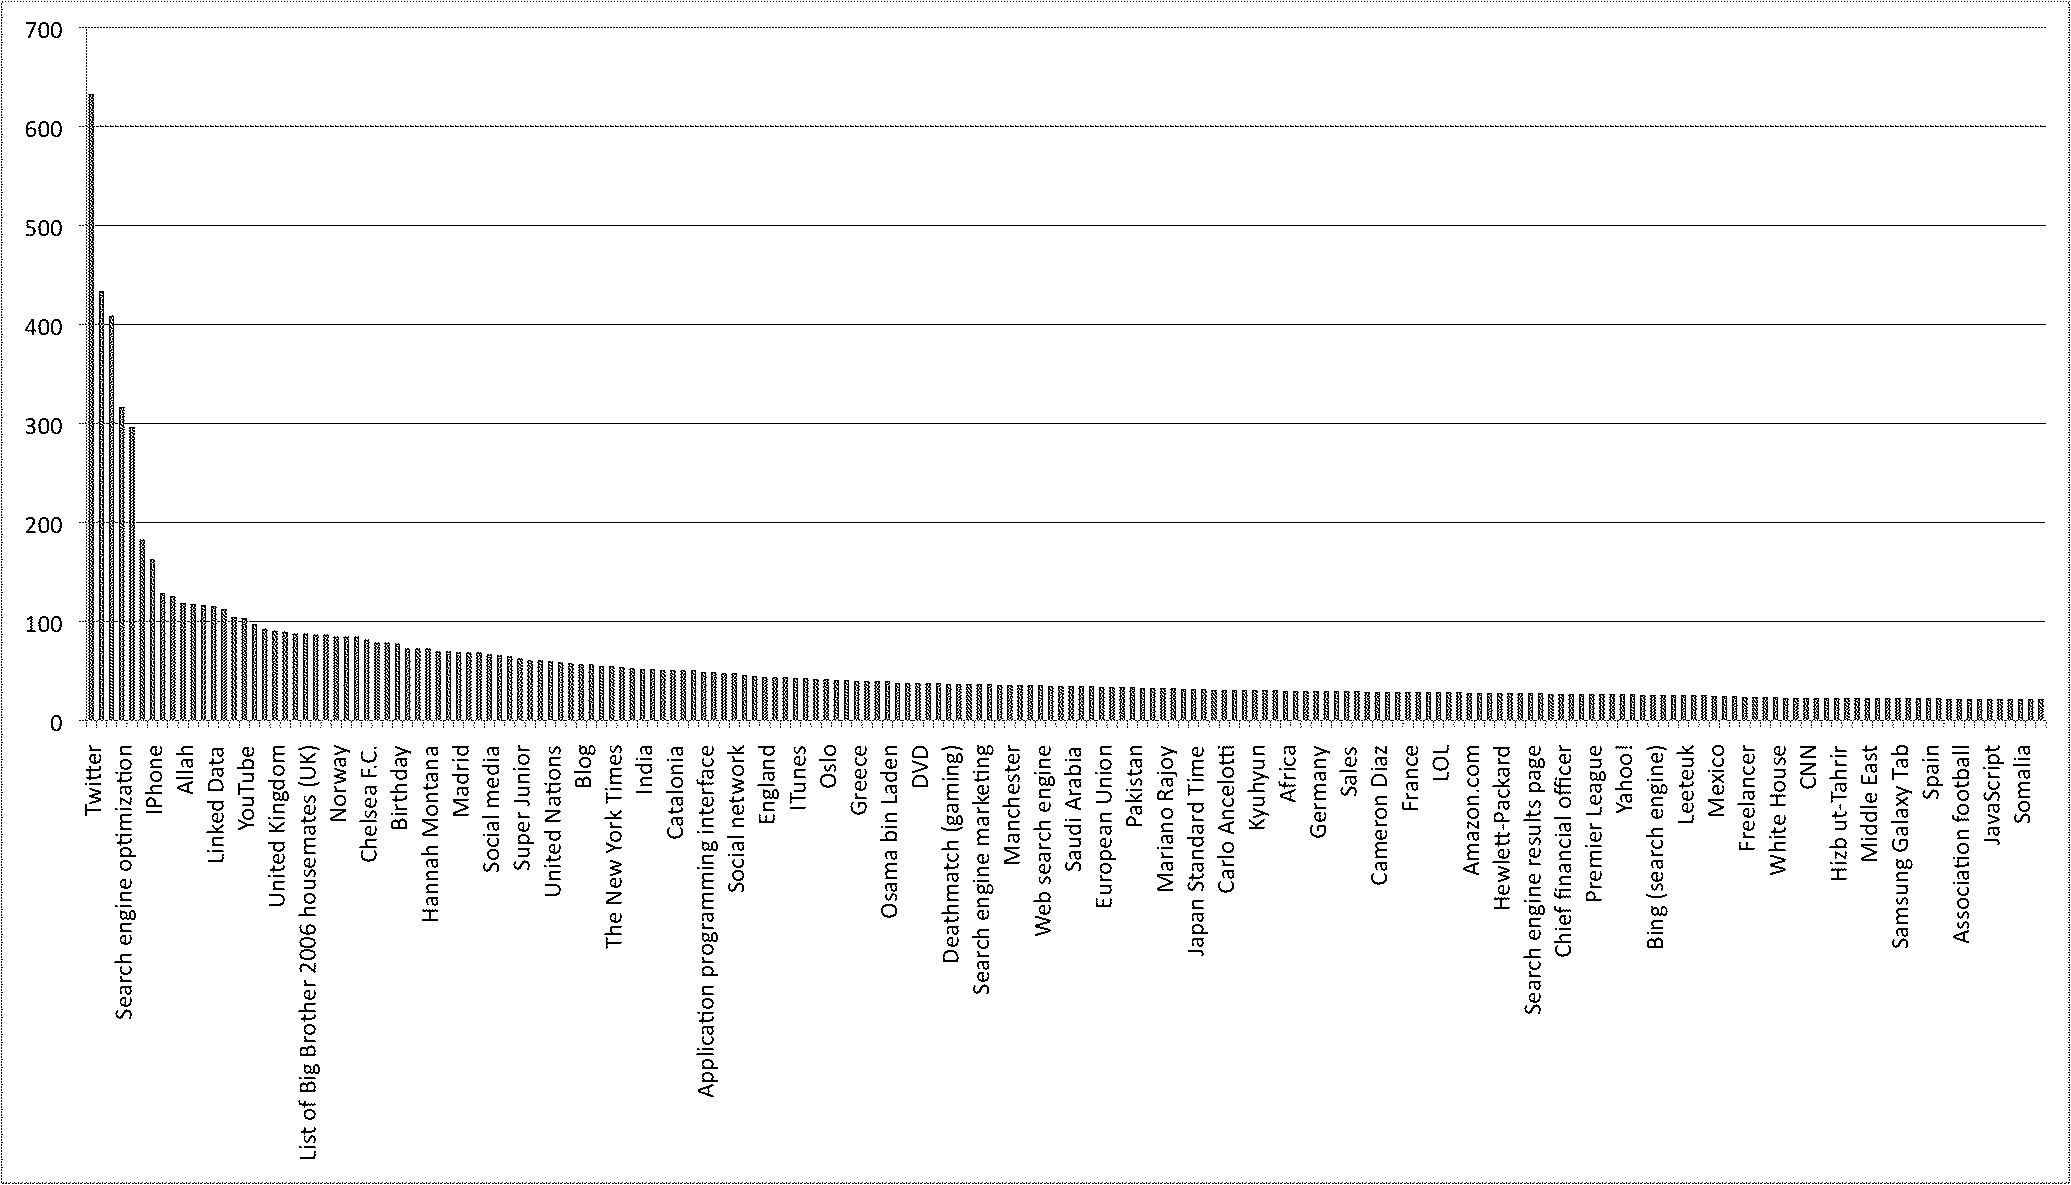
\includegraphics[width=1.0\linewidth]{./resources/twittertopentities.png}
\caption{Twitter top entities as reported by Twitter Swarm NLP users.}
\label{fig:twittertopentities}
\end{figure*}

\begin{table}
\begin{center}
    \begin{tabular}{ | l | l |}
    \hline
	\textbf{Country} & \textbf{Visits} \\ \hline
	Germany	& 2,280 \\ \hline
	Thailand & 2,133 \\ \hline
	Mexico & 1,586 \\ \hline
	Czech Republic & 1,416 \\ \hline
	United Kingdom & 1,100 \\ \hline
	India & 1,047 \\ \hline
	Australia & 854 \\ \hline
	Indonesia	& 826 \\ \hline
	Italy & 805 \\ \hline
	United States & 742 \\
    \hline
    \end{tabular}
\end{center}
\caption{Top-10 locations of users of the Facebook Swarm NLP browser extension (May 1 -- Nov. 12).}
\label{tab:facebooklocations}        
\end{table}

\begin{table}
\begin{center}
    \begin{tabular}{ | l | l |}
    \hline
	\textbf{Country} & \textbf{Visits} \\ \hline
	United States & 831 \\ \hline
	Japan & 296 \\ \hline
	Germany & 288 \\ \hline
	Italy & 284 \\ \hline
	Finland & 204 \\ \hline
	United Kingdom & 200 \\ \hline
	Australia & 176 \\ \hline
	Russia & 162 \\ \hline
	Thailand & 155 \\ \hline
	Spain & 147 \\
    \hline
    \end{tabular}
\end{center}
\caption{Top-10 locations of users of the Twitter Swarm NLP browser extension (May 1 -- Nov. 12).}
\label{tab:twitterlocations}        
\end{table}

\section{Discussion}
% Talk about what network to use for what purpose, talk about brand analysis etc.

% Twitter
% Total Events 35,958
% Unique Events 27,594  

% Facebook
% Total Events 316,910 
% Unique Events 136,196 

% http://dbpedia.org/resource/Eid_Mubarak http://dbpedia.org/resource/Eid_ul-Fitr
% http://dbpedia.org/resource/Celcom Malaysia

\section{Related Work} \label{sec:relatedwork}
We report on related work separated into the fields of:
\begin{itemize}
\item \emph{semantic annotation of microposts}, which focuses on named entity detection and disambiguation;
\item \emph{trend or popularity detection}, which is based on term frequencies;
\item \emph{commercialization of social data}, which aims at monetization of gathered insights.
\end{itemize}
The presented examples are not to be seen as \emph{the} standard selection of relevant works, but rather as representative overview on a plethora of very similar publications and services.
In addition to that, we also provide a \emph{comparison with micropost author-focused approaches} of our work.

\subsection{Semantic Annotation of Microposts}
Passant \textit{et al.} introduced a Semantic MicroBlogging (\textit{sic}) framework~(SMOB,~\cite{Passant2008}) that enables a \textit{distributed, open, and semantic} microblogging experience based on Semantic Web and Linked Data technologies by annotating microposts with common vocabularies such as FOAF or SIOC.
SMOB relies on distributed autonomous hubs that communicate with each other to exchange microposts and subscriptions, which can also be cross-posted to Twitter.
The authors suggest the use of meaningful hashtags such as \texttt{\#dbp:Eiffel\_Tower}, or \texttt{\#geo:Paris\_France}, in the style of RDF prefixes for DBpedia and GeoNames.

In the Linked Open Social Signals project~(LOSS,~\cite{Mendes:LOSS}), Mendes \textit{et al.} investigate the representation of microposts as Linked Open Data and address the problem of information overload caused by the sheer amount of microposts (the authors call the opinions, observations, and suggestions contained in microposts ``social signals'', hence the project name).
While the micropost community has come up with hashtags in order to categorize microposts.
These hashtags are ambiguous and have to be explicitly added to the micropost by the author and due to length constraints are sometimes left out in favor of more text.
The main goal of LOSS is thus to enable collective analysis of social signals for sense-making by using Linked Open Data principles in combination with realtime push models.

\subsection{Trend and Popularity Detection}
As outlined before, research on trend and popularity detection has mainly focused on Twitter due to the facile availability of data through the Twitter Streaming API.
A basic overview is given by by Benhardus in~\cite{benhardus2010streaming}, where the author applies and evaluates several methodologies to large Twitter corpora such as (normalized) term frequency, TF-IDF, and entropy.
With TwitterMonitor~\cite{Mathioudakis:2010:TTD:1807167.1807306}, Mathioudakis and Koudas present a \textit{bursty} keyword-based Twitter trend detector demonstration.
Their algorithm is able to detect groups of bursty keywords and also enrich trends with potentially associated keywords.
Trendsmap provides a realtime mapping of Twitter trends across the world.
The service allows for splitting up one's view in different granularity levels by current location, city, region, and world.

\subsection{Commercialization of Social Data}
``What the Trend''~\cite{whatthetrend} is a service that provides manually curated and annotated reports on Twitter top-trending topics.
The service adds explanations to why tropics trend and data behind trending patterns.
Primarily the information on ``What the Trend'' is user-generated, however, the service also sells curated yearly reports.

Topsy Labs, Inc. offers a commercial API~\cite{topsy} that allows for \textit{applying social intelligence to realtime decisioning}.
Therefore, the service applies algorithms that try to rank popular videos, photos, blog posts, and news stories, most influential users on a certain topic, and individual user influence scores.
Supported social networks include Twitter and Google+.
Different from the social networks themselves, Topsy Labs claims to allowing for going back in history up to the year 2008 with their commercial API.

Twimpact \cite{twimpact} is a realtime Twitter data analysis company with special focus on social media communication that reports \textit{immediate events, current trends and relevant opinion leaders} within social media conversations.
Twimpact uses machine learning-based ranking techniques that do not rely on simple reader/follower counts, but rather include actual communication patterns, such as retweets. 

\subsection{Comparison with Micropost Author-focused Approaches}
With our focus on micropost readers rather than on micropost authors, we strive for a paradigm shift with important consequences.
The first and most important consequence is the availability of only a limited set of micropost data, as illustrated by the Venn diagram in~\autoref{fig:vennreadunread}.
Only a subset (of unknown size) of all microposts that get authored also ever gets read.
Where the Twitter Streaming API offers up to 10\% coverage of all authored tweets, full access to the firehose with 100\% coverage of all authored tweets is handled through Twitter data providers~\cite{dataproviders}.
For Facebook, no such publicly available option exists.
For obvious reasons, there is no API from either of the networks for read microposts, which is why we came up with the idea to hook into the reading experience on social networks through browser extensions.
The second consequence has to do with privacy issues.
While aggregated public data, as made possible by accessing it via APIs, may feel like violating privacy~\cite{nyt}, it is still public data.
However, the approach we took in this paper goes one step further by explicitly accessing a social network user's timeline, and reporting back named entities to a Web analytics service (the same that gets used already by Twitter). 
It is important to note, however, that no connection is been made between a user's individual timeline and the person behind.
We have stated all accessed data in the extension descriptions.
The third consequence is the potential bias introduced by targeting one specific Web browser with the extensions.
Ideally, we would target all major browsers, however, due to scalability reasons, currently we can only target one browser.

\begin{figure}
\centering
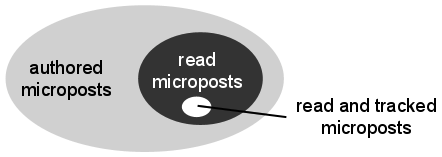
\includegraphics[width=0.4\linewidth]{./resources/vennreadunread.png}
\caption{Only a subset (of unknown size) of all microposts that get authored also ever get read.}
\label{fig:vennreadunread}
\end{figure}

\section{Future Work and Conclusion} \label{sec:futureworkandconclusion}

%%%%%%%%%%% The bibliography starts:
\bibliographystyle{abbrv}
\bibliography{swj2012}

\end{document}